\documentclass[twocolumn]{article}
\usepackage{graphicx}
\usepackage{amsmath}
\usepackage{url}

\begin{document}
For a system defined with many possible configurations defined through a model Hamiltonian, calculated from model potentials, or through first principles methods it may be desirable to calculate the density of energy states $G(E_j)$. With the energy density of states the partition function,
\begin{equation}
\begin{split}
Z = \sum_{i}^{\Omega}e^{\frac{-e_i}{k_B T} }= \sum_{j}^{\Pi}G(E_j)e^{\frac{-E_j}{k_BT}} \;,
\end{split}
\end{equation}
 can be exactly calculated an from it many important properties of interest determined. Properties of interest calculated from the partition function include  free energy, entropy, specific hear, and ensemble averages. One method of solving this problem has been temperature dependent simulations involving  Metropolis algorithm and histogram re weighting techniques\cite{landau_MC_simulations}.  Another algorithm called the  Wang and Landau algorithm\cite{WL_phys_rev_lett} has been developed which is temperature independent.  In this paper a method is proposed that combines the use of random sets along with the importance sampling method of the Wang and Landau algorithm. This algorithm is referred to as the ``B$_{L}$ENDER" (B$_{L}$end Each New Density Each Round) algorithm. The name ``B$_{L}$ENDER" functions as an acronym and adjective which comes in part because how it blends the ideas of a random set and the Wang and Landau method, and also due to the nature of the algorithm iteratively blending histograms to produce a converged density of states. The purpose of developing the ``B$_{L}$ENDER" algorithm was to work towards an algorithm that is both accurate and trivial  to parallelize. The Wang and Landau method does have parallel versions, including  restricting random walkers to specific energy ranges or allowing the walkers to explore the entire space while periodically communicating with each other \cite{MP_Wang_Landau,P_imp_Wang_Landau, Hframe_Wang_Landau}. The ``B$_{L}$ENDER" is trivial to parallelize as it is based on a set of random walkers than each can explore the entire energy range. It is hoped that due to the ``B$_{L}$ENDER" being presented in the form of sets that the mathematics of set theory and real analysis can be used to analyze the algorithm and possibly further extended its capabilities from those presented in this work. 

In a previous paper the notion of the master set $\{ \Sigma_i, e_i \}_\Omega $ of the $\Omega$ total configurations and energies was put forth. The master set refers to the actual configurations of the defined system. In practice to calculate the density of energy states $G(E_j)$  may be possible through randomly sampling the configurations space.  In a previous work it was shown that a properly scaled histogram of a sampled set $\{ \Sigma_s, e_s \}_\mathcal{S}$ converges to the exact density of states $G(E_j)$ as the the number of samples $\mathcal{S}$ goes to infinity. The problem with this method is that if $\Omega$ is large, which it is for many problems,  then the computationally effort to achieve convergence is not feasible.  This work tackles this issue produce an algorithm that is highly parallel in terms of the calculations of the energies  but also incorporates importance sampling such as in the Wang and Landau method. 

The ``B$_{L}$ENDER" algorithm proposed in this work  is given as follows. It is noted that the following algorithm is in terms of producing a relative density of states $H(E_j)$.  \\
\begin{equation}
\begin{split}
&1.\hspace{0.125cm} H(E_j)^i ,\hspace{0.15cm}  \{\Sigma_{s},e_s\}_{\mathcal{S}}^i\\
&2. \hspace{0.125cm}\{\Sigma_{s},e_s\}_{\mathcal{S}}^i \rightarrow  \{\Sigma_{s}^{'},e_s^{'}\}_{\mathcal{S}}^i\\
&3. \hspace{0.125cm}H(E_j)^{Ii} = H(E_j)^i + \mathcal{H}(E_j, \{e_{s}^{'}\}_{\mathcal{S}}^i) \\
&4. \hspace{0.125cm} \Sigma_{s}^{i'} \rightarrow \Sigma_{s}^{i+1}, \hspace{0.15cm} P(1, H(e_s)^{Ii}/H(e_s^{'})^{Ii})\\
& \hspace{0.125cm}else  \hspace{0.15cm} \Sigma_{s}^i \rightarrow \Sigma_{s}^{i+1}\\
&5. \hspace{0.125cm} H(E_j)^{i+1} = H(E_j)^{i} + C_o\mathcal{H}(E_j, \{e_s\}_{\mathcal{S}}^{i+1})\frac{H(E_j)^{Ii}}{\sum_j H(E_j)^{Ii} }\\
%&6. \hspace{0.125cm} N = \sum_j G(E_j)^{i+1} \hspace{0.125cm}\\
%& if \hspace{0.125cm} G(E_j)^{i+1}\frac{\Omega}{N}  < 1, \hspace{0.125cm}  G(E_j)^{i+1} = G(E_j)^{i+1} \frac{N}{\Omega}
\end{split}
\end{equation}
Where  $H(E_j)^0 \equiv \mathcal{H}(E_j,\{e_s\}_{\mathcal{S}}^0)$ with $\mathcal{H}(E_j,\{e_s\}_{\mathcal{S}})$ being a histogram function that counts the number of energies $E_j$ in the set $\{e_s\}_{\mathcal{S}}$. In this work $\{\Sigma_{s},e_s\}_{\mathcal{S}}^0$  are a randomly(uniformly) drawn set from the configuration space $\{ \Sigma_i, e_i \}_\Omega $. In the second step  a random change is applied to each element of the sampled set $\{\Sigma_{s},e_s\}_{\mathcal{S}}^i$ to produced a ``perturbed" set $ \{\Sigma_{s}^{'},e_s^{'}\}_{\mathcal{S}}^i$ , for the Ising model this could be randomly flipping a spin. In the third step a histogram of the ``perturbed" set is added to the current estimate of the density of states $H(E_j)^i$ to produce an intermediary density of states $H(E_j)^{Ii}$. In the fourth step a random number is drawn between zero and one for every sampled configuration, if this number is less then the ratio of the density of states $H(e_s)^{Ii}/H(e_s^{'})^{Ii}$ then the perturbed configuration $\Sigma_{s}^{'i}$ goes to $\Sigma_{s}^{i+1}$,  else the unperturbed configuration $\Sigma_{s}^{i}$ goes to $\Sigma_{s}^{i+1}$. In the fifth step a histogram of the updated $\{ e_s \}^{i+1}$ energies is made and added (blended) in to the current density of states $H(E_j)^i$   by multiplying  by a constant(which effects convergence) and the relative probability of each energy $E_j$ in the the intermediary density of states $H(E_j)^{Ii}$. After the algorithm is deemed to be complete it is necessary to re-normalize the iterated relative density of states $H(E_j)^f$ at the final iteration $f$ as follows, 
\begin{equation}
\begin{split}
&1. \hspace{0.125cm} A = \sum_jH(E_j)^f\\
&2. \hspace{0.125cm} G(E_j)\approx H(E_j)^f \frac{\Omega}{A} \;,
\end{split}
\end{equation}
to produce the properly normalized estimated value of $G(E_j)$. 

In this work the algorithm discussed is tested using the 2-d zero field ferromagnetic Ising model. The total energy of a square 2-d Ising model of dimension  $n\times n$ with periodic boundary conditions is given by, 
\begin{equation}
e_i = -J\sum_{k,l =1}^n \sigma^i_{k,l} 
\left( \sigma^i_{k+1,l} + \sigma^i_{k,l+1}
\right). \label{2D}
\end{equation}
Where $e_i$ denotes the i'th energy of the set  $\{\Sigma_i, e_i \}_{\Omega} $ configurations and energies. The configurations and energies of the 2-d Ising model are inherently defined by the lattice site spin variables $\sigma^i_{k,l}$ and coupling constant $J$. In this work $J=1$. Several tests of the algorithm will be performed. A test of the convergence properties with respect to the number of samples $\mathcal{S}$. A test of the convergence properties in terms of the size of the system determined by $n$. These test will utilize comparisons to the exact results. Also a qualitative understanding of the convergence as a function of time will be presented. 
The first test is a test to show the convergence of the algorithm in terms of the number of samples $\mathcal{S}$ and the number of iterations of the algorithm. To test the accuracy of the simulations the results will be compared to the exact result solved by Beale \cite{Beale_2d_ising}. The accuracy of the simulation will be determined by, 
\begin{equation}
\epsilon(I,o)  = \frac{1}{\Pi} \sum_{j=1}^{\Pi}\frac{|\ln(G_{ex}(E_j))- \ln(G_{bl}(E_j,I,o))|}{\ln(G_{ex}(E_j))}\; . 
\end{equation}

Where $G_{ex}(E_j)$ is the exact density of states, $G_{bl}(E_j,I,o)$ is the density of states at iteration number $I$ from initial conditions and trajectory $o$.
To test the convergence in terms of number of samples $\mathcal{S}$ and number of iterations $I$ for $n=12$.  The simulations where done until iteration average,
\begin{equation}
\mathcal{E} \equiv \langle \hspace{0.1cm} \epsilon(I,o)\hspace{0.1cm}\rangle_{I} = \frac{1}{I}\int_{0}^{I}\epsilon(I^{'},o)dI^{'} \;,
\end{equation}
 was less then 1$\%$, the corresponding number of iterations was recorded, this was then repeated for multiple simulations. The average value of $I$ over initial configurations and trajectories that produced a specific  value of $\mathcal{E}=c$ equal  was then calculated to give, 
\begin{equation}
 \mathcal{I}(\mathcal{E}=c) \equiv \langle \hspace{0.1cm}  I(\mathcal{E} = c) \hspace{0.1cm}\rangle_{o} \;.
 \end{equation}
 It is noted that the error is only well defined when all of the possible
 energies have been located. In Fig \ref{its_to_err}(a)  it is shown how the number of iterations needed to achieve $\mathcal{E}=1\%$ scales with the number of samples for a 12$\times$12 system, for visual purposes the x-axis is on a natural log scale. Another interesting scaling property is the number of iterations necessary to find all of the energies in the system, this is shown in Fig \ref{its_to_err}(b). 
\begin{figure}
(a)\\
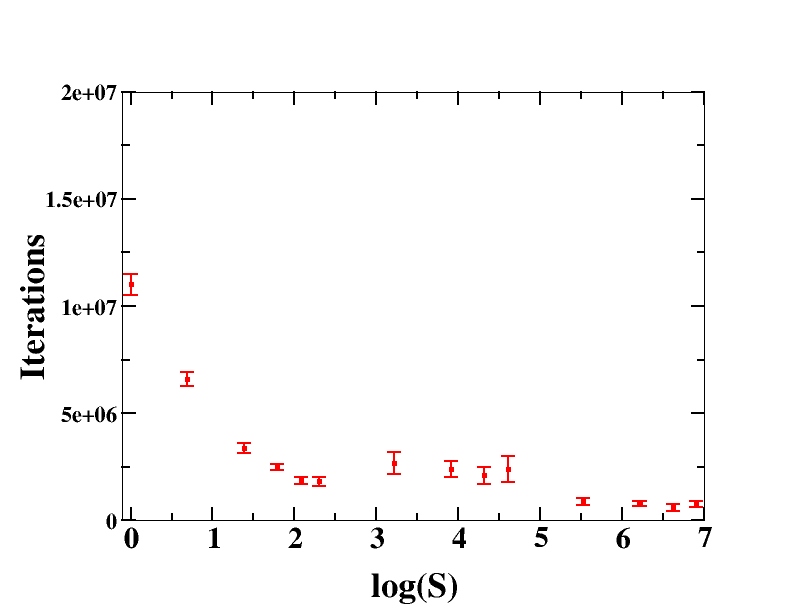
\includegraphics[width=8cm]{its_for_err.png}
\caption{\label{its_to_err} (a) average number of iterations($\mathcal{I}$) necessary to achieve $\mathcal{E}=1\%$ and (b) average number of iterations($\mathcal{I}$) necessary
to find all of the energies. Each for a for a 12X12 system. }
\end{figure}

 
\bibliography{Bib}
\bibliographystyle{unsrt}


\end{document}
